% the sample map
\begin{figure}
  \centering
  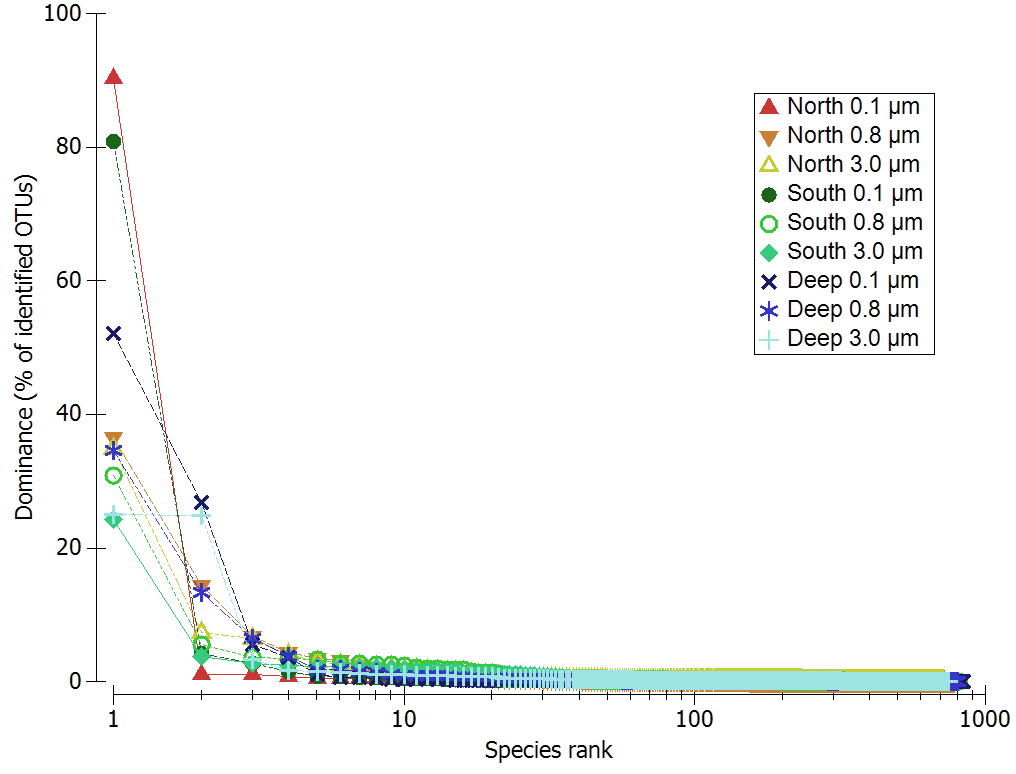
\includegraphics[width=\textwidth]{../polarfront/rankabundance.png}
  \caption[Rank-abundance curves for OTUs in each zone and size fraction]{Rank-abundance curves for OTUs identified in each zone and size fraction. The dominance of a given OTU is calculated as its relative abundance as a percentage of the relative abundance of all identified OTUs. The x-axis is scaled logarithmically.}
  \label{fig:rankabundance}
\end{figure}
